\section{Initial Experimentation - Classification}
Here we report our initial experiments where we formulated the task of predicting near-collision time as a classification model. 

\subsection{Binary Classification: What happens 1 second into the future?}

In initial experimentation, we formulated the task as binary classification whether there is a near-collision in next one second or not. The output layer in Fig. \ref{fig:model} is replaced by a two-neuron layer followed by softmax function. The binary cross entropy loss is used to train the network. An alternative naive way to solve this task is to compare the foot of pedestrians' bounding boxes with a predefined threshold on pixel's vertical image coordinate. The Table \ref{tab:binary_classification} compares the F1 score from our learning approach versus the naive baseline. F1 score is the harmonic mean of precision and recall and thus higher F1 score is more accurate. For the naive baseline, if the foot of the pedestrian lies in the lower $37.5\%$ (empirically found to be best) of the vertical size of image, we classify it as collision within one second.  \\

We use GradCAM \cite{gradCAM} to see which part of the image our trained network attends to. The attention maps of few test examples are shown in Figures \ref{fig:gradcam1}, \ref{fig:gradcam2}.
% \begin{align*}

%     L^{c} = ReLU(\sum_{k} \alpha_{k}^{c}A_{k})\\
%     y_c: \text{Score for the class $c$}\\
%     {\alpha_k}^{c}: \text{Weight for $k^{th}$ channel in last convolutional map for class $c$}\\
%     A_{ij}^{k}: \text{Activation of $(i, j)$ in $k^{th}$ convolutional channel}\\
%     L^{c}: \text{Heatmap for class $c$}
% \end{align*}
It first computes the gradient of the score $y^{c}$ for a class $c$ with respect to the activations of last convolutional layer. The gradients are global-average-pooled to get the importance of a feature map $k$ for class $c$, denoted as ${\alpha_k}^{c}$.
$$
    {\alpha_k}^{c} = \frac{1}{Z}\sum_{i}\sum_{j}\frac{\delta y^{c}}{\delta {A_{ij}}^{k}} 
$$
A weighted combination of forward activation maps is finally upsampled to the  size of input image to visualize the attention map. 
\begin{align*}
    L^{c} = ReLU(\sum_{k} \alpha_{k}^{c}A_{k})\\
   % y_c: \text{Score for the class $c$}\\
    {\alpha_k}^{c}: \text{Weight for $k^{th}$ channel in last convolutional map for class $c$}\\
    A_{ij}^{k}: \text{Activation of $(i, j)$ in $k^{th}$ convolutional channel}\\
    L^{c}: \text{Attention map for class $c$}
\end{align*}
The confusion matrix over a test set passed through the trained network is reported in table \ref{tab:confusion_matrix}. To tackle the data imbalance between the collision instances (2106) and no collision instances (8579), a weighted sampler is used in training with collision instances having a weight of $0.6$ and no collision instances having a lower weight of $0.4$.
%% I should balance the training! 

    \begin{figure}[ht]
      \centering
      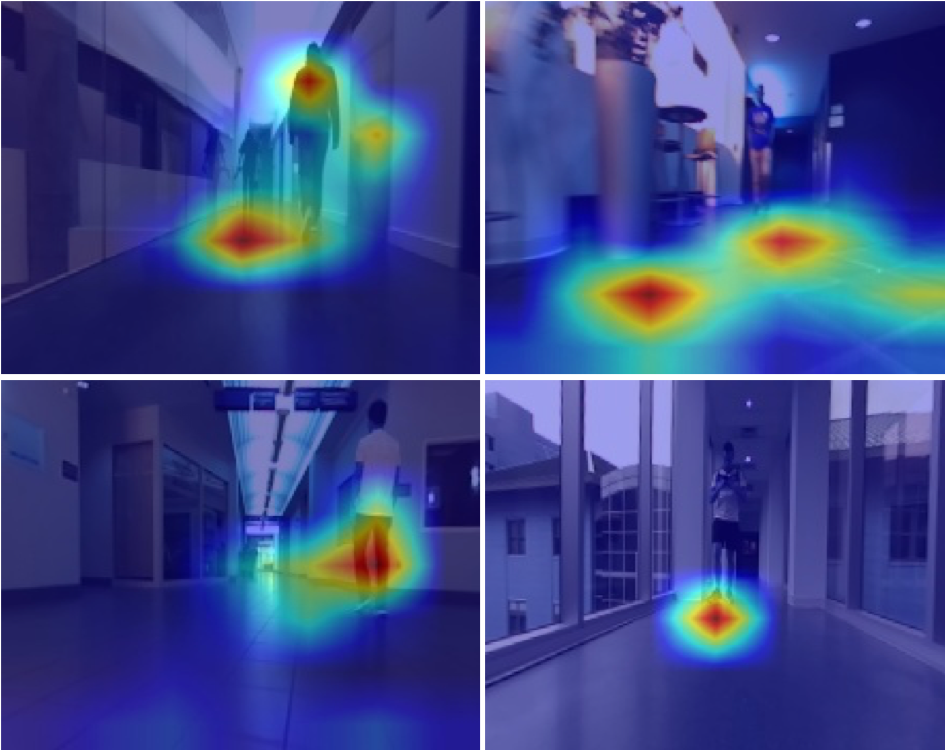
\includegraphics[height=8cm, width=\columnwidth]{figs/grad_binary_class.png}
      \caption{Visualization of attention maps using GradCAM; Top Left: Two Persons going away, Top Right: One person with two probable trajectories, Bottom Left: A person going away, Bottom Right: A person approaching}
      \label{fig:gradcam1}
  \end{figure}

    \begin{figure}[ht]
      \centering
      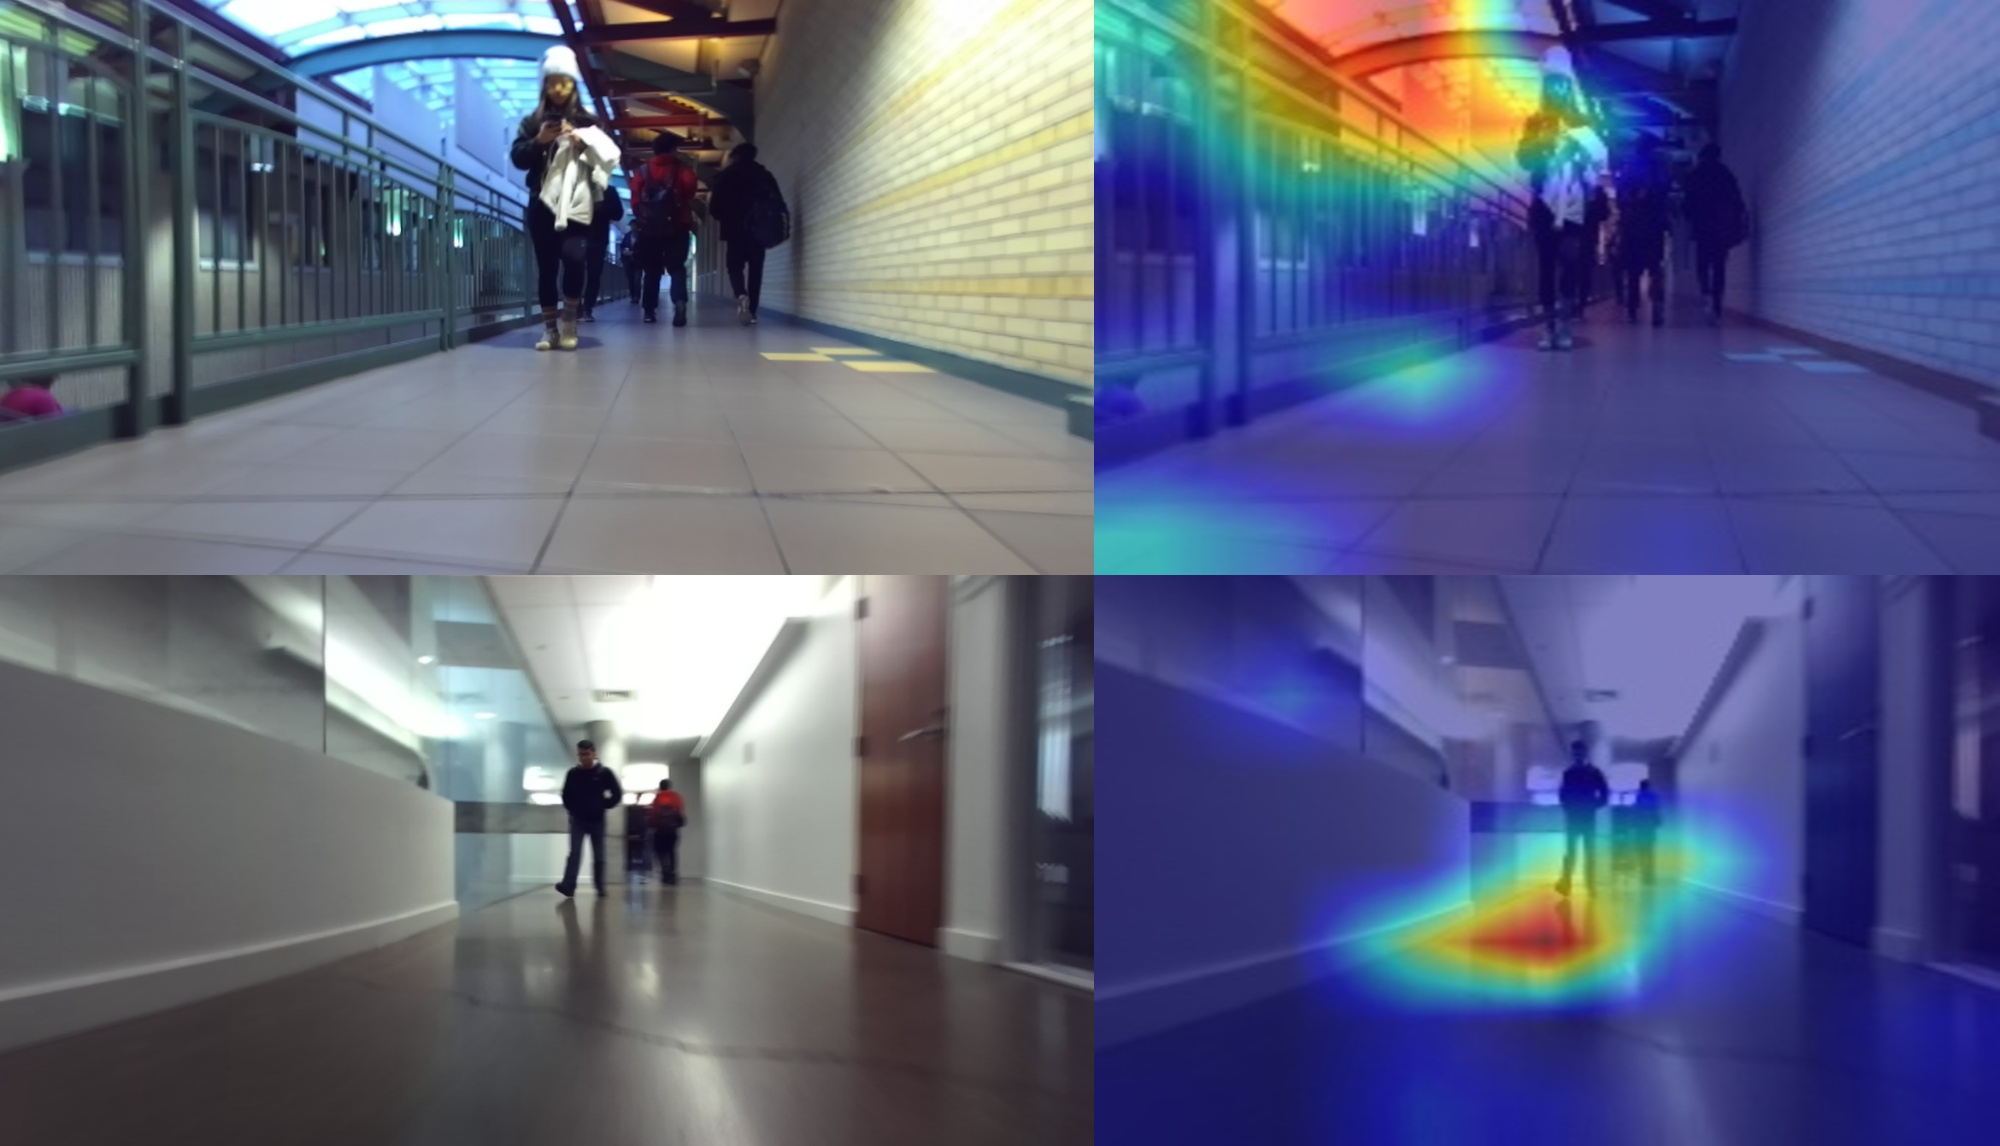
\includegraphics[height=8cm, width=\columnwidth]{figs/gradCAM.pdf}
      \caption{Left: RGB Image, Right: Corresponding GradCAM}
      \label{fig:gradcam2}
  \end{figure}

\begin{table}[h]
\caption{Confusion Matrix from Binary Classification}\label{tab:confusion_matrix}
\noindent
\renewcommand\arraystretch{1.5}
\setlength\tabcolsep{0pt}
\begin{tabular}{c >{\bfseries}r @{\hspace{0.7em}}c @{\hspace{0.4em}}c @{\hspace{0.7em}}l}
  \multirow{10}{*}{\parbox{1.1cm}{\bfseries\raggedleft Actual\\ value}} & 
    & \multicolumn{2}{c}{\bfseries Prediction outcome} & \\
  & & \bfseries \small{collision} & \bfseries \small{no collision} \\
  & \small{collision} & \MyBox{634}{} & \MyBox{36}{} \\[2.4em]
  & \small{no collision} & \MyBox{53}{} & \MyBox{2840}{}  
\end{tabular}
\end{table}

\begin{table}[h]
\caption {Near-Collision Prediction formulated as Binary Classification: F1 Scores from our approach compared with a naive baseline} \label{tab:binary_classification} 
\begin{tabular}{|P{0.45\textwidth}|P{0.45\textwidth}|} \hline
Method  &  F1 Score \\ \hline
Naive baseline $(0.625 Y)$ & 0.8488 \\ \hline 
N-stream VGG $(N = 4)$ &  \textbf{0.9344} \\ \hline %% From slides  
\end{tabular}
\end{table}

\subsection{Multi-label Classification}
On previous task of binary classification for 0-1 sec, our deep learning approach performs better than the naive thresholding as reported in Table \ref{tab:binary_classification}. We thus move on to increasing the difficulty of the task, i.e, a multi-label classification problem where we classify if there is going to be a near-collision instance in (1) within a second, (2) between 1-2 seconds, (2) between 2-3 seconds or (4) no collision within 3 seconds. Our training and test data distribution for this multi-label classfication is provided in Table \ref{tab:class_distribution}. For training, we used multilabel soft margin loss \cite{pytorch} as the loss function. The F1 scores reported in Table \ref{tab:multi_label_classification} indicate that the naive baseline can give better predictions within 2 seconds into the future while the proposed multilabel deep neural network performs better for the latter classes, i.e., predictions in the range 2-3 seconds and no collision instances. One of the challenges of this multi-label formulation over the regression formulation is that we have to empirically decide a threshold on the confidence score for each class to classify it as the positive or negative label. The precision-recall curve or area under ROC curve \cite{roc} can be used to evaluate the performance of the trained model at different thresholds and then decide the best threshold accordingly. \\

\begin{table}[h]
\caption {Class Distribution} \label{tab:class_distribution} 
\begin{tabular}{|P{0.3\textwidth}|P{0.3\textwidth}|P{0.3\textwidth}|} \hline
Near-Collision Time  &  Training Data & Test Data \\ \hline
0-1 s &  4150 & 287 \\ \hline 
1-2 s &  2590 & 185 \\ \hline
2-3 s &  2185 & 169 \\ \hline
After 3 s & 13049  & 507 \\ \hline 
\end{tabular}
\end{table}

\begin{table}[h]
\caption {Near-Collision Prediction formulated as Multi-Class Classification} \label{tab:multi_label_classification} 
\begin{tabular}{|P{4cm}|P{4cm}|P{3cm}|P{3cm}|} \hline
Near-Collision Time  &  Vertical Image Coordinate for naive baseline $Y = 720$  & F1 Score from Naive Baseline & F1 Score from N-Stream VGG \\ \hline
0-1 s & $> 0.625Y$ &  0.849 & 0.759 \\ \hline 
1-2 s & $> 0.560Y$ & 0.720 & 0.630 \\ \hline
2-3 s & $> 0.520Y$ & \textbf{0.629} & \textbf{0.947} \\ \hline
After 3 s & $\le 0.520Y$ & \textbf{0.522}  & \textbf{0.620} \\ \hline 
\end{tabular}
\end{table}
 
 
  \begin{figure*}[ht]
      \centering
      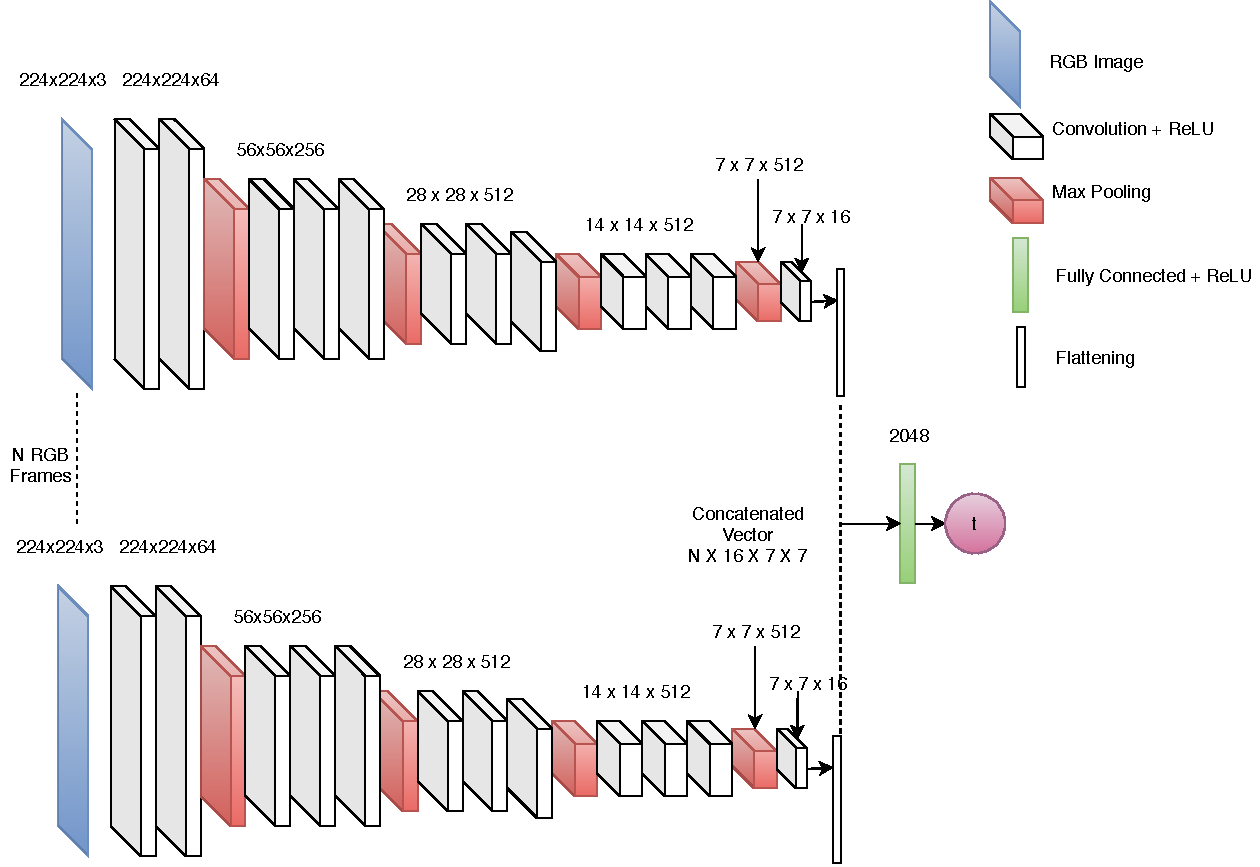
\includegraphics[height=7.0cm, width=12cm]{figs/vgg_2.pdf}
      \caption{Our model with VGG-16 as backbone where the final output is time to collision denoted as $t$ }
      \label{fig:model}
  \end{figure*}

\section{Regression Experiments - Different temporal windows as input}
Overcoming the limitations of classification formulation, we move on to regression formulation which performed better as previously explained in chapter \ref{chap:approach}. \\

We now describe our evaluation procedure to decide the optimum temporal window as input on two different video network architectures. We further compare the performance with strong collision prediction baselines.
A single image can capture spatial information but no motion characteristics. Thus, we propose to use a sequence of image frames as history.  By feeding $N$ image frames, we consider a history of $\frac{N-1}{10}$ seconds. The temporal window of input frames was gradually increased from 2 frames (0.1 sec) to 9 frames (0.8 sec). To quantify the performance, we measure the mean absolute error (MAE) for the predictions on the test set and the standard deviation in error. From Table \ref{tab:hist}, it is empirically concluded to use a temporal window of 0.5 seconds, i.e, 6 frames for most accurate predictions. 

\begin{table}[ht]
\caption{Distribution of absolute error (mean $\pm$ std) on near-collision dataset using different number of input frames}\label{tab:hist}
\begin{tabular}{|P{0.3\textwidth}|P{0.3\textwidth}|P{0.3\textwidth}|} \hline
Number of frames & Multi-stream VGG  & I3D  \\ \hline 
1 & 0.879 $\pm$ 0.762s & 0.961 $\pm$ 0.707s  \\ \hline
2 & 0.828 $\pm$  0.739s & 0.879 $\pm$ 0.665s \\ \hline 
3 & 0.826  $\pm$  0.647s & 0.914 $\pm$ 0.659s \\ \hline 
4  & 0.866 $\pm$  0.696s & \textbf{0.811 $\pm$ 0.642s}  \\ \hline
5 & 0.849 $\pm$ 0.734 & 0.849 $\pm$ 0.734s \\ \hline 
6  & \textbf{0.753 $\pm$ 0.687s} & 0.816 $\pm$ 0.663s   \\ \hline
7 & 0.757 $\pm$  0.722s & 0.848 $\pm$ 0.733s \\ \hline
8 & 0.913 $\pm$ 0.732s & 0.811 $\pm$ 0.647s \\ \hline 
9 & 0.817 $\pm$  0.738s & 0.855 $\pm$ 0.670s \\ \hline
\end{tabular}
\end{table}

\section{Experimental comparison of architectures}
We show a comparison of the performance of multi-stream VGG model and baselines including state-of-the-art methods in Table \ref{tab:baselines}. 

\begin{table}[ht]
\caption {Distribution of absolute error (mean $\pm$ std) on regression task compared with different baselines} \label{tab:baselines} 
\begin{tabular}{|P{6cm}|P{3cm}|P{2.25cm}|} \hline
Method  &  Mean (in s) & Std (in s)\\ \hline
Constant baseline ($\mathbb{E}[y_{true}]$) & 1.382 & 0.839\\ \hline 
Tracking + Linear Model \cite{BBeep} &  1.055  & 0.962 \\ \hline 
DroNet \cite{DroNet} & 1.099 &  0.842  \\ \hline 
Gandhi et al \cite{gandhi} & 0.884 & 0.818 \\ \hline
Single Image VGG-16 & 0.879  & 0.762 \\ \hline
I3D (4 frames) \cite{i3d} & 0.811  & 0.642  \\ \hline
\textbf{Multi-stream VGG (6 frames)} & \textbf{0.753}  & \textbf{0.687}  \\ \hline 
\end{tabular}
\end{table}

  \begin{figure}[ht]
      \centering
      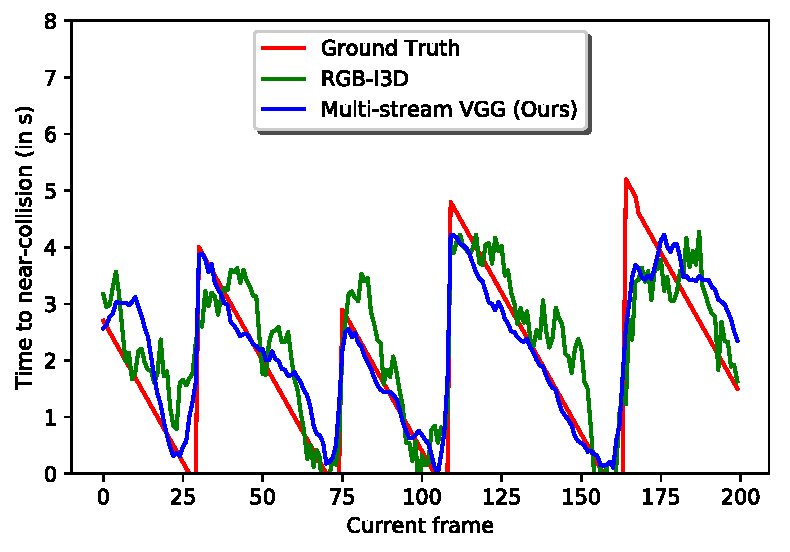
\includegraphics[height=7.5cm, width=\textwidth]{figs/400_new.pdf}
      \caption{Prediction of multi-stream VGG is smoother than I3D. The discontinuities here arise in the absence of pedestrians.}
      \label{fig:plot}
  \end{figure}
  
    \begin{figure*}[ht]
      \centering
      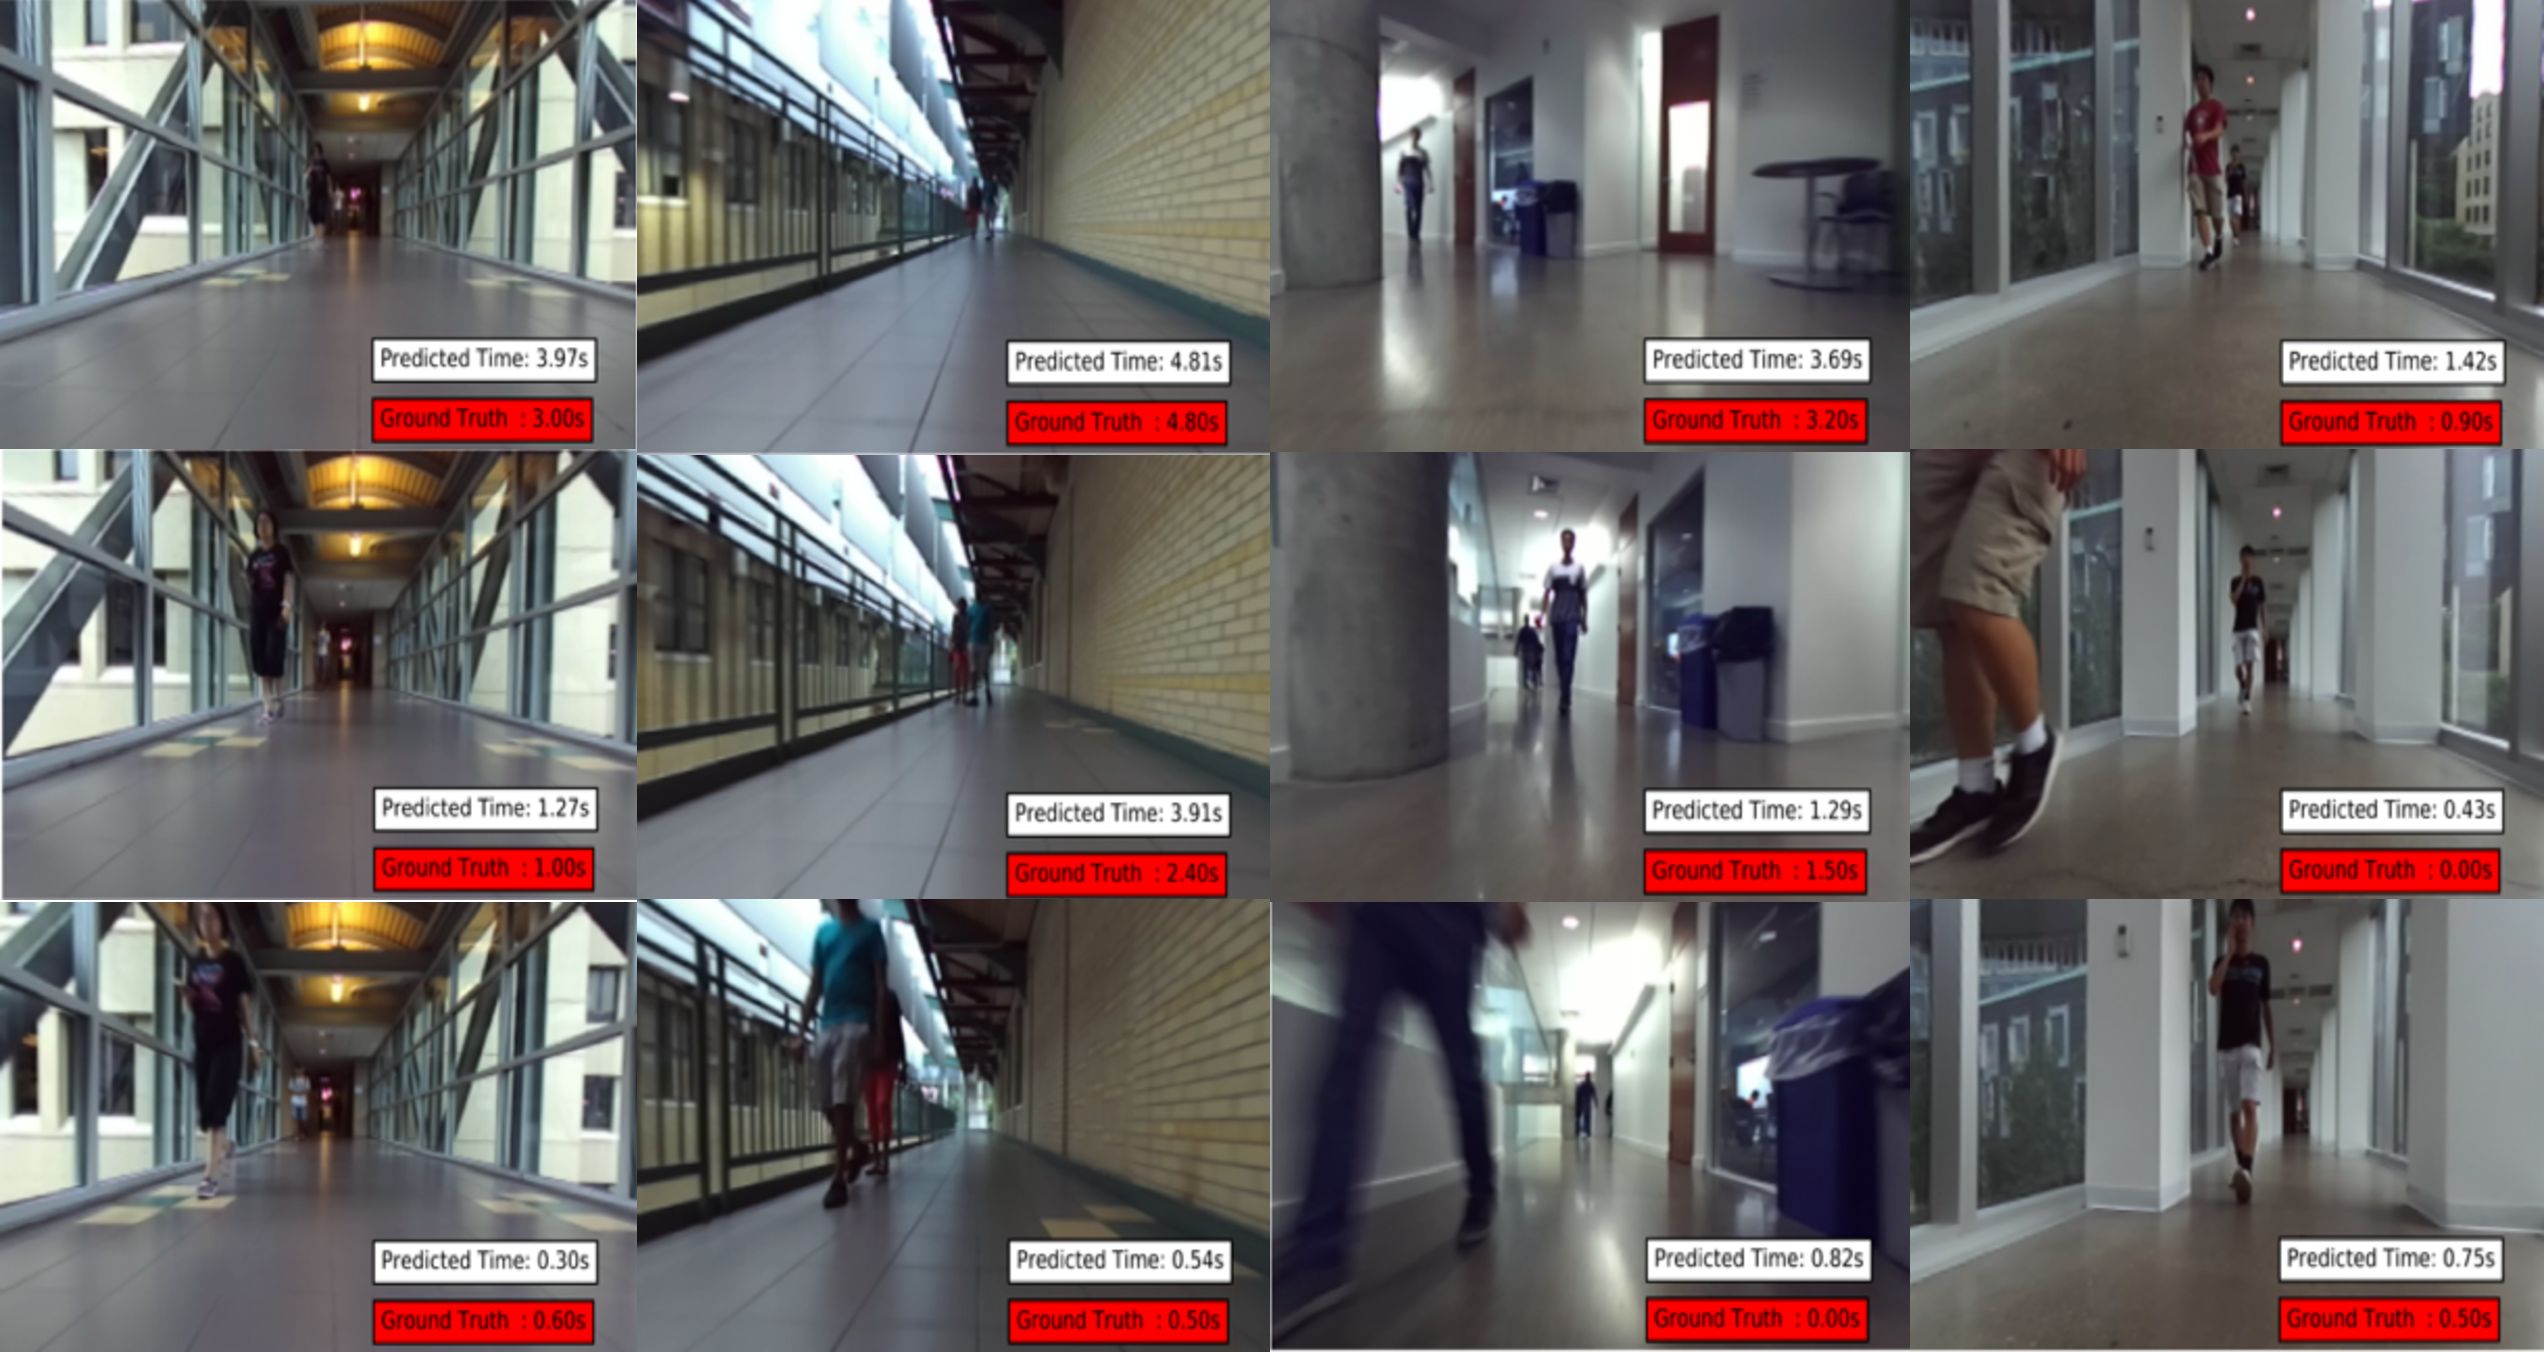
\includegraphics[height=10cm,width=\textwidth]{figs/qr2.pdf}
      \caption{Predictions on four different test videos}
      \label{fig:testVideos}
  \end{figure*}


\begin{enumerate}
    \item \textit{Constant Baseline:} On the training data of 12,620 samples, we compute the mean time to proximity denoted by $\mathbb{E}[y_{true}]$ as a weak baseline. For each test input, we predict $\mathbb{E}[y_{true}]$ which was found to be $2.23$ seconds. 
    
    \item \textit{Tracking followed by constant velocity model:} In dynamic environments, pedestrians are often tracked using a stereo camera or LIDAR. By saving few previous locations (0.5-2 seconds), a linear regression fit is used to predict the velocity vector of person \cite{BBeep}, \cite{SIPP}. This velocity vector is then linearly extrapolated to predict where the pedestrian will be over the next 6 seconds and the corresponding accuracy is reported in Table \ref{tab:baselines}. A major disadvantage in this method is the need for image-based tracking which is less reliable at low framerate of $10$ fps.     
    \item \textit{Deep learning for collision avoidance:} Collision avoidance using deep learning has been previously proposed in \cite{gandhi} and \cite{DroNet}. Gandhi et al \cite{gandhi} created a UAV crash dataset to train AlexNet for classifying the current image into one of these three categories of drone policy: go straight, turn left or turn right. For learning time to near-collision using their approach, we take a single image as input and use AlexNet architecture with ImageNet-pretrained weights as initialization. The only difference lies in the output layer which is a single neuron regression instead of a three-neuron classifier. Our multi-stream VGG outperformed current-frame AlexNet as reported in Table \ref{tab:baselines}.
    
ResNet-8 architecture used in DroNet \cite{DroNet} takes in the single image and after the last ReLU layer splits into two fully-connected streams outputting steering angle and collision probability respectively. To experiment with their learning approach, we used ResNet-8 architecture with only one output, i.e., time to near-collision. The performance is close to the constant velocity prediction model as reported in Table \ref{tab:baselines} and thus it can be seen that it is unable to leverage real-world data. One of the reasons for its low performance could be the unavailability of ImageNet-pretrained weights for ResNet-8 architecture and thus it has to be trained from scratch on our proximity dataset which is much smaller than the Udacity's car-driving dataset of 70,000 images used for training steering angle stream in DroNet.   
    
    %% should elaborate in related work 
    %% Here only the network architecture and why is it chosen as a baseline 
    \item \textit{I3D for action classification in videos:} Two-Stream Inflated 3D ConvNet (I3D) \cite{i3d} is a strong baseline to learn a task from videos. All the $ N \times N$ filters and pooling kernels in ImageNet-pretrained Inception-V1 network \cite{inceptionv1} are inflated with an additional temporal dimension to become $N \times N \times N$. I3D has two streams - one trained on RGB inputs and other on optical flow inputs. To avoid adding the latency of optical flow computation for real-time collision forecasting, we only used the RGB stream of I3D. We fine-tuned the I3D architecture which was pre-trained on Kinetics Human Action Video dataset \cite{i3d} on our near-collision dataset by sending $N$ RGB frames as input where $N = \{1,2, \hdots, 8,9\}$ as reported in Table \ref{tab:hist}. The outermost layer is modified from 400-neuron classifier to 1-neuron regressor. Since our $N$-frame input is smaller than the original implementation on 64-frame input, we decreased the temporal stride of last max-pool layer from 2 to 1. While 6 input frames were found to be the best for proposed multi-stream VGG network, we experimented again with the optimal history on I3D. The performance of I3D with varying number of input frames is reported in Table \ref{tab:hist}.  For $N = 4, 6, 8$, I3D is found to give the best results among 1-9 frames though our multi-stream VGG prediction for $N = 6$ outperformed the I3D prediction in best case. 
\end{enumerate}
\section{Qualitative Evaluation}
% After seeing quantitative results as reported in Table \ref{tab:baselines}, the mean absolute error between proposed approach and the closest baseline I3D differs by a small number of 0.05 seconds. Does it mean that the proposed method offers only a slight improvement over existing approaches which might be negligible during real-time execution? To answer this we plotted the predictions made by proposed network and most competitive baseline I3D to compare with the ground truth. 
From the plots shown in Fig. \ref{fig:plot} we can observe that the predictions given by multi-stream VGG on 6 frames give smoother output as compared to undesired fluctuations in I3D output. We also qualitatively show in Fig. \ref{fig:testVideos} the comparison of time to near-collision predicted by our method vs the ground truth. 
%This motivates the introduction of another evaluation metric - smoothness factor. 
